\documentclass[1p]{elsarticle_modified}
%\bibliographystyle{elsarticle-num}

%\usepackage[colorlinks]{hyperref}
%\usepackage{abbrmath_seonhwa} %\Abb, \Ascr, \Acal ,\Abf, \Afrak
\usepackage{amsfonts}
\usepackage{amssymb}
\usepackage{amsmath}
\usepackage{amsthm}
\usepackage{scalefnt}
\usepackage{amsbsy}
\usepackage{kotex}
\usepackage{caption}
\usepackage{subfig}
\usepackage{color}
\usepackage{graphicx}
\usepackage{xcolor} %% white, black, red, green, blue, cyan, magenta, yellow
\usepackage{float}
\usepackage{setspace}
\usepackage{hyperref}

\usepackage{tikz}
\usetikzlibrary{arrows}

\usepackage{multirow}
\usepackage{array} % fixed length table
\usepackage{hhline}

%%%%%%%%%%%%%%%%%%%%%
\makeatletter
\renewcommand*\env@matrix[1][\arraystretch]{%
	\edef\arraystretch{#1}%
	\hskip -\arraycolsep
	\let\@ifnextchar\new@ifnextchar
	\array{*\c@MaxMatrixCols c}}
\makeatother %https://tex.stackexchange.com/questions/14071/how-can-i-increase-the-line-spacing-in-a-matrix
%%%%%%%%%%%%%%%

\usepackage[normalem]{ulem}

\newcommand{\msout}[1]{\ifmmode\text{\sout{\ensuremath{#1}}}\else\sout{#1}\fi}
%SOURCE: \msout is \stkout macro in https://tex.stackexchange.com/questions/20609/strikeout-in-math-mode

\newcommand{\cancel}[1]{
	\ifmmode
	{\color{red}\msout{#1}}
	\else
	{\color{red}\sout{#1}}
	\fi
}

\newcommand{\add}[1]{
	{\color{blue}\uwave{#1}}
}

\newcommand{\replace}[2]{
	\ifmmode
	{\color{red}\msout{#1}}{\color{blue}\uwave{#2}}
	\else
	{\color{red}\sout{#1}}{\color{blue}\uwave{#2}}
	\fi
}

\newcommand{\Sol}{\mathcal{S}} %segment
\newcommand{\D}{D} %diagram
\newcommand{\A}{\mathcal{A}} %arc


%%%%%%%%%%%%%%%%%%%%%%%%%%%%%5 test

\def\sl{\operatorname{\textup{SL}}(2,\Cbb)}
\def\psl{\operatorname{\textup{PSL}}(2,\Cbb)}
\def\quan{\mkern 1mu \triangleright \mkern 1mu}

\theoremstyle{definition}
\newtheorem{thm}{Theorem}[section]
\newtheorem{prop}[thm]{Proposition}
\newtheorem{lem}[thm]{Lemma}
\newtheorem{ques}[thm]{Question}
\newtheorem{cor}[thm]{Corollary}
\newtheorem{defn}[thm]{Definition}
\newtheorem{exam}[thm]{Example}
\newtheorem{rmk}[thm]{Remark}
\newtheorem{alg}[thm]{Algorithm}

\newcommand{\I}{\sqrt{-1}}
\begin{document}

%\begin{frontmatter}
%
%\title{Boundary parabolic representations of knots up to 8 crossings}
%
%%% Group authors per affiliation:
%\author{Yunhi Cho} 
%\address{Department of Mathematics, University of Seoul, Seoul, Korea}
%\ead{yhcho@uos.ac.kr}
%
%
%\author{Seonhwa Kim} %\fnref{s_kim}}
%\address{Center for Geometry and Physics, Institute for Basic Science, Pohang, 37673, Korea}
%\ead{ryeona17@ibs.re.kr}
%
%\author{Hyuk Kim}
%\address{Department of Mathematical Sciences, Seoul National University, Seoul 08826, Korea}
%\ead{hyukkim@snu.ac.kr}
%
%\author{Seokbeom Yoon}
%\address{Department of Mathematical Sciences, Seoul National University, Seoul, 08826,  Korea}
%\ead{sbyoon15@snu.ac.kr}
%
%\begin{abstract}
%We find all boundary parabolic representation of knots up to 8 crossings.
%
%\end{abstract}
%\begin{keyword}
%    \MSC[2010] 57M25 
%\end{keyword}
%
%\end{frontmatter}

%\linenumbers
%\tableofcontents
%
\newcommand\colored[1]{\textcolor{white}{\rule[-0.35ex]{0.8em}{1.4ex}}\kern-0.8em\color{red} #1}%
%\newcommand\colored[1]{\textcolor{white}{ #1}\kern-2.17ex	\textcolor{white}{ #1}\kern-1.81ex	\textcolor{white}{ #1}\kern-2.15ex\color{red}#1	}

{\Large $\underline{12a_{0515}~(K12a_{0515})}$}

\setlength{\tabcolsep}{10pt}
\renewcommand{\arraystretch}{1.6}
\vspace{1cm}\begin{tabular}{m{100pt}>{\centering\arraybackslash}m{274pt}}
\multirow{5}{120pt}{
	\centering
	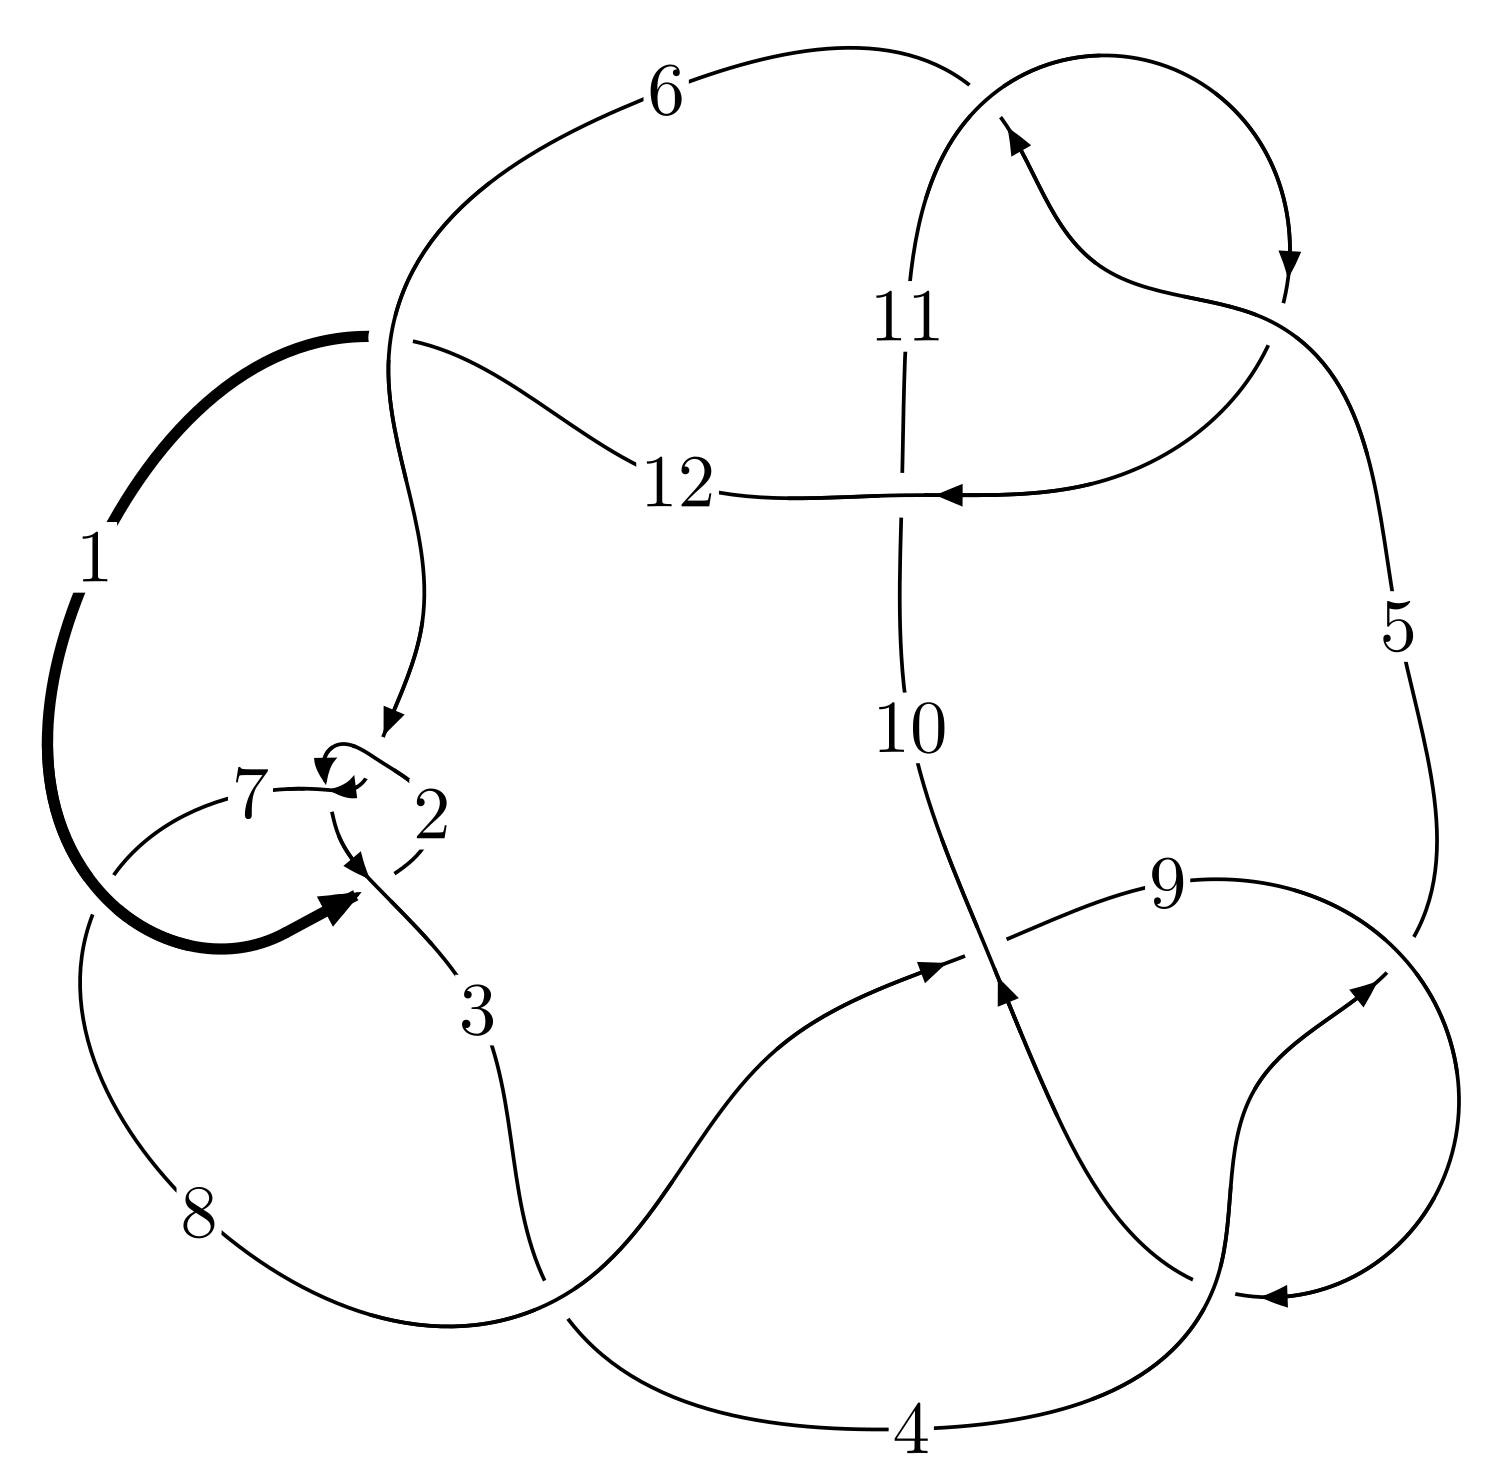
\includegraphics[width=112pt]{../../../GIT/diagram.site/Diagrams/png/1316_12a_0515.png}\\
\ \ \ A knot diagram\footnotemark}&
\allowdisplaybreaks
\textbf{Linearized knot diagam} \\
\cline{2-2}
 &
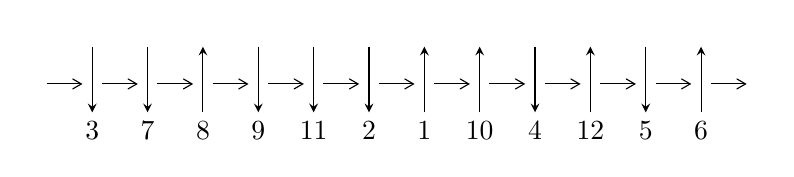
\begin{tikzpicture}[x=20pt, y=17pt]
	% nodes
	\node (C0) at (0, 0) {};
	\node (C1) at (1, 0) {};
	\node (C1U) at (1, +1) {};
	\node (C1D) at (1, -1) {3};

	\node (C2) at (2, 0) {};
	\node (C2U) at (2, +1) {};
	\node (C2D) at (2, -1) {7};

	\node (C3) at (3, 0) {};
	\node (C3U) at (3, +1) {};
	\node (C3D) at (3, -1) {8};

	\node (C4) at (4, 0) {};
	\node (C4U) at (4, +1) {};
	\node (C4D) at (4, -1) {9};

	\node (C5) at (5, 0) {};
	\node (C5U) at (5, +1) {};
	\node (C5D) at (5, -1) {11};

	\node (C6) at (6, 0) {};
	\node (C6U) at (6, +1) {};
	\node (C6D) at (6, -1) {2};

	\node (C7) at (7, 0) {};
	\node (C7U) at (7, +1) {};
	\node (C7D) at (7, -1) {1};

	\node (C8) at (8, 0) {};
	\node (C8U) at (8, +1) {};
	\node (C8D) at (8, -1) {10};

	\node (C9) at (9, 0) {};
	\node (C9U) at (9, +1) {};
	\node (C9D) at (9, -1) {4};

	\node (C10) at (10, 0) {};
	\node (C10U) at (10, +1) {};
	\node (C10D) at (10, -1) {12};

	\node (C11) at (11, 0) {};
	\node (C11U) at (11, +1) {};
	\node (C11D) at (11, -1) {5};

	\node (C12) at (12, 0) {};
	\node (C12U) at (12, +1) {};
	\node (C12D) at (12, -1) {6};
	\node (C13) at (13, 0) {};

	% arrows
	\draw[->,>={angle 60}]
	(C0) edge (C1) (C1) edge (C2) (C2) edge (C3) (C3) edge (C4) (C4) edge (C5) (C5) edge (C6) (C6) edge (C7) (C7) edge (C8) (C8) edge (C9) (C9) edge (C10) (C10) edge (C11) (C11) edge (C12) (C12) edge (C13) ;	\draw[->,>=stealth]
	(C1U) edge (C1D) (C2U) edge (C2D) (C3D) edge (C3U) (C4U) edge (C4D) (C5U) edge (C5D) (C6U) edge (C6D) (C7D) edge (C7U) (C8D) edge (C8U) (C9U) edge (C9D) (C10D) edge (C10U) (C11U) edge (C11D) (C12D) edge (C12U) ;
	\end{tikzpicture} \\
\hhline{~~} \\& 
\textbf{Solving Sequence} \\ \cline{2-2} 
 &
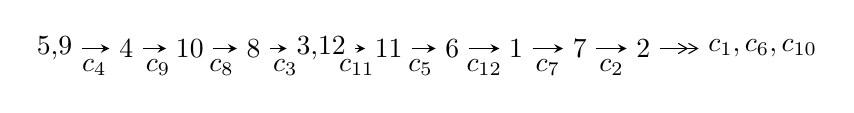
\begin{tikzpicture}[x=23pt, y=7pt]
	% node
	\node (A0) at (-1/8, 0) {5,9};
	\node (A1) at (1, 0) {4};
	\node (A2) at (2, 0) {10};
	\node (A3) at (3, 0) {8};
	\node (A4) at (65/16, 0) {3,12};
	\node (A5) at (41/8, 0) {11};
	\node (A6) at (49/8, 0) {6};
	\node (A7) at (57/8, 0) {1};
	\node (A8) at (65/8, 0) {7};
	\node (A9) at (73/8, 0) {2};
	\node (C1) at (1/2, -1) {$c_{4}$};
	\node (C2) at (3/2, -1) {$c_{9}$};
	\node (C3) at (5/2, -1) {$c_{8}$};
	\node (C4) at (7/2, -1) {$c_{3}$};
	\node (C5) at (37/8, -1) {$c_{11}$};
	\node (C6) at (45/8, -1) {$c_{5}$};
	\node (C7) at (53/8, -1) {$c_{12}$};
	\node (C8) at (61/8, -1) {$c_{7}$};
	\node (C9) at (69/8, -1) {$c_{2}$};
	\node (A10) at (11, 0) {$c_{1},c_{6},c_{10}$};

	% edge
	\draw[->,>=stealth]	
	(A0) edge (A1) (A1) edge (A2) (A2) edge (A3) (A3) edge (A4) (A4) edge (A5) (A5) edge (A6) (A6) edge (A7) (A7) edge (A8) (A8) edge (A9) ;
	\draw[->>,>={angle 60}]	
	(A9) edge (A10);
\end{tikzpicture} \\ 

\end{tabular} \\

\footnotetext{
The image of knot diagram is generated by the software ``\textbf{Draw programme}" developed by Andrew Bartholomew(\url{http://www.layer8.co.uk/maths/draw/index.htm\#Running-draw}), where we modified some parts for our purpose(\url{https://github.com/CATsTAILs/LinksPainter}).
}\phantom \\ \newline 
\centering \textbf{Ideals for irreducible components\footnotemark of $X_{\text{par}}$} 
 
\begin{align*}
I^u_{1}&=\langle 
b- u,\;u^{33}+u^{32}+\cdots+4 a+1,\;u^{34}+9 u^{32}+\cdots+2 u+1\rangle \\
I^u_{2}&=\langle 
-3.29206\times10^{15} u^{57}+7.29251\times10^{15} u^{56}+\cdots+6.43771\times10^{15} b+1.37987\times10^{16},\;u^{57}- u^{56}+\cdots+a-8,\\
\phantom{I^u_{2}}&\phantom{= \langle  }u^{58}- u^{57}+\cdots-8 u+1\rangle \\
I^u_{3}&=\langle 
b+u,\;a^2+2 a u- a- u,\;u^2+1\rangle \\
\\
\end{align*}
\raggedright * 3 irreducible components of $\dim_{\mathbb{C}}=0$, with total 96 representations.\\
\footnotetext{All coefficients of polynomials are rational numbers. But the coefficients are sometimes approximated in decimal forms when there is not enough margin.}
\newpage
\renewcommand{\arraystretch}{1}
\centering \section*{I. $I^u_{1}= \langle b- u,\;u^{33}+u^{32}+\cdots+4 a+1,\;u^{34}+9 u^{32}+\cdots+2 u+1 \rangle$}
\flushleft \textbf{(i) Arc colorings}\\
\begin{tabular}{m{7pt} m{180pt} m{7pt} m{180pt} }
\flushright $a_{5}=$&$\begin{pmatrix}1\\0\end{pmatrix}$ \\
\flushright $a_{9}=$&$\begin{pmatrix}0\\u\end{pmatrix}$ \\
\flushright $a_{4}=$&$\begin{pmatrix}1\\- u^2\end{pmatrix}$ \\
\flushright $a_{10}=$&$\begin{pmatrix}- u\\u^3+u\end{pmatrix}$ \\
\flushright $a_{8}=$&$\begin{pmatrix}- u^3\\u^5+u^3+u\end{pmatrix}$ \\
\flushright $a_{3}=$&$\begin{pmatrix}- u^6- u^4+1\\u^8+2 u^6+2 u^4\end{pmatrix}$ \\
\flushright $a_{12}=$&$\begin{pmatrix}-\frac{1}{4} u^{33}-\frac{1}{4} u^{32}+\cdots-\frac{11}{4} u-\frac{1}{4}\\u\end{pmatrix}$ \\
\flushright $a_{11}=$&$\begin{pmatrix}-\frac{1}{4} u^{33}-\frac{1}{4} u^{32}+\cdots-\frac{7}{4} u-\frac{1}{4}\\u\end{pmatrix}$ \\
\flushright $a_{6}=$&$\begin{pmatrix}-\frac{1}{4} u^{33}+\frac{1}{4} u^{32}+\cdots+\frac{1}{4} u+\frac{5}{4}\\u^2\end{pmatrix}$ \\
\flushright $a_{1}=$&$\begin{pmatrix}-\frac{1}{4} u^{33}-\frac{1}{4} u^{32}+\cdots-\frac{7}{4} u-\frac{1}{4}\\u^5+u^3+u\end{pmatrix}$ \\
\flushright $a_{7}=$&$\begin{pmatrix}\frac{7}{4} u^{33}+\frac{5}{4} u^{32}+\cdots+\frac{23}{4} u+\frac{7}{4}\\-\frac{1}{4} u^{33}-\frac{1}{4} u^{32}+\cdots+\frac{1}{4} u-\frac{1}{4}\end{pmatrix}$ \\
\flushright $a_{2}=$&$\begin{pmatrix}-\frac{1}{2} u^{33}-\frac{1}{2} u^{32}+\cdots-\frac{7}{2} u-\frac{1}{2}\\-\frac{1}{4} u^{33}-\frac{1}{4} u^{32}+\cdots+\frac{1}{4} u-\frac{1}{4}\end{pmatrix}$\\&\end{tabular}
\flushleft \textbf{(ii) Obstruction class $= -1$}\\~\\
\flushleft \textbf{(iii) Cusp Shapes $= -6 u^{33}+u^{32}-53 u^{31}+5 u^{30}-234 u^{29}+9 u^{28}-642 u^{27}-13 u^{26}-1183 u^{25}-104 u^{24}-1454 u^{23}-276 u^{22}-1067 u^{21}-433 u^{20}-162 u^{19}-423 u^{18}+569 u^{17}-178 u^{16}+658 u^{15}+134 u^{14}+288 u^{13}+280 u^{12}-22 u^{11}+188 u^{10}-106 u^9+30 u^8-52 u^7-40 u^6-19 u^5-35 u^4-2 u^3-11 u^2-5 u-4$}\\~\\
\newpage\renewcommand{\arraystretch}{1}
\flushleft \textbf{(iv) u-Polynomials at the component}\newline \\
\begin{tabular}{m{50pt}|m{274pt}}
Crossings & \hspace{64pt}u-Polynomials at each crossing \\
\hline $$\begin{aligned}c_{1}\end{aligned}$$&$\begin{aligned}
&u^{34}+15 u^{33}+\cdots-3 u+4
\end{aligned}$\\
\hline $$\begin{aligned}c_{2},c_{6}\end{aligned}$$&$\begin{aligned}
&u^{34}-3 u^{33}+\cdots-3 u+2
\end{aligned}$\\
\hline $$\begin{aligned}c_{3},c_{12}\end{aligned}$$&$\begin{aligned}
&u^{34}+3 u^{33}+\cdots+48 u+32
\end{aligned}$\\
\hline $$\begin{aligned}c_{4},c_{5},c_{9}\\c_{11}\end{aligned}$$&$\begin{aligned}
&u^{34}+9 u^{32}+\cdots+2 u+1
\end{aligned}$\\
\hline $$\begin{aligned}c_{7}\end{aligned}$$&$\begin{aligned}
&u^{34}-9 u^{33}+\cdots-13 u+6
\end{aligned}$\\
\hline $$\begin{aligned}c_{8},c_{10}\end{aligned}$$&$\begin{aligned}
&u^{34}-18 u^{33}+\cdots-4 u+1
\end{aligned}$\\
\hline
\end{tabular}\\~\\
\newpage\renewcommand{\arraystretch}{1}
\flushleft \textbf{(v) Riley Polynomials at the component}\newline \\
\begin{tabular}{m{50pt}|m{274pt}}
Crossings & \hspace{64pt}Riley Polynomials at each crossing \\
\hline $$\begin{aligned}c_{1}\end{aligned}$$&$\begin{aligned}
&y^{34}+9 y^{33}+\cdots-225 y+16
\end{aligned}$\\
\hline $$\begin{aligned}c_{2},c_{6}\end{aligned}$$&$\begin{aligned}
&y^{34}-15 y^{33}+\cdots+3 y+4
\end{aligned}$\\
\hline $$\begin{aligned}c_{3},c_{12}\end{aligned}$$&$\begin{aligned}
&y^{34}-29 y^{33}+\cdots+12544 y+1024
\end{aligned}$\\
\hline $$\begin{aligned}c_{4},c_{5},c_{9}\\c_{11}\end{aligned}$$&$\begin{aligned}
&y^{34}+18 y^{33}+\cdots+4 y+1
\end{aligned}$\\
\hline $$\begin{aligned}c_{7}\end{aligned}$$&$\begin{aligned}
&y^{34}-3 y^{33}+\cdots+563 y+36
\end{aligned}$\\
\hline $$\begin{aligned}c_{8},c_{10}\end{aligned}$$&$\begin{aligned}
&y^{34}+2 y^{33}+\cdots-12 y+1
\end{aligned}$\\
\hline
\end{tabular}\\~\\
\newpage\flushleft \textbf{(vi) Complex Volumes and Cusp Shapes}
$$\begin{array}{c|c|c}  
\text{Solutions to }I^u_{1}& \I (\text{vol} + \sqrt{-1}CS) & \text{Cusp shape}\\
 \hline 
\begin{aligned}
u &= -0.325102 + 0.931137 I \\
a &= \phantom{-}3.02864 - 0.12001 I \\
b &= -0.325102 + 0.931137 I\end{aligned}
 & \phantom{-}2.90695 + 0.12402 I & \phantom{-}1.68955 - 3.89611 I \\ \hline\begin{aligned}
u &= -0.325102 - 0.931137 I \\
a &= \phantom{-}3.02864 + 0.12001 I \\
b &= -0.325102 - 0.931137 I\end{aligned}
 & \phantom{-}2.90695 - 0.12402 I & \phantom{-}1.68955 + 3.89611 I \\ \hline\begin{aligned}
u &= \phantom{-}0.379532 + 0.974939 I \\
a &= -2.71723 + 0.31509 I \\
b &= \phantom{-}0.379532 + 0.974939 I\end{aligned}
 & \phantom{-}3.60419 - 5.09535 I & \phantom{-}3.52400 + 9.16731 I \\ \hline\begin{aligned}
u &= \phantom{-}0.379532 - 0.974939 I \\
a &= -2.71723 - 0.31509 I \\
b &= \phantom{-}0.379532 - 0.974939 I\end{aligned}
 & \phantom{-}3.60419 + 5.09535 I & \phantom{-}3.52400 - 9.16731 I \\ \hline\begin{aligned}
u &= -0.545074 + 0.928759 I \\
a &= \phantom{-}1.93949 + 0.24437 I \\
b &= -0.545074 + 0.928759 I\end{aligned}
 & -2.30189 + 4.06636 I & -5.42219 - 5.57604 I \\ \hline\begin{aligned}
u &= -0.545074 - 0.928759 I \\
a &= \phantom{-}1.93949 - 0.24437 I \\
b &= -0.545074 - 0.928759 I\end{aligned}
 & -2.30189 - 4.06636 I & -5.42219 + 5.57604 I \\ \hline\begin{aligned}
u &= \phantom{-}0.578615 + 0.697678 I \\
a &= -1.53750 - 0.18162 I \\
b &= \phantom{-}0.578615 + 0.697678 I\end{aligned}
 & -3.69260 - 4.93095 I & -7.79856 + 7.85932 I \\ \hline\begin{aligned}
u &= \phantom{-}0.578615 - 0.697678 I \\
a &= -1.53750 + 0.18162 I \\
b &= \phantom{-}0.578615 - 0.697678 I\end{aligned}
 & -3.69260 + 4.93095 I & -7.79856 - 7.85932 I \\ \hline\begin{aligned}
u &= \phantom{-}0.512199 + 1.009370 I \\
a &= -2.07083 + 0.50301 I \\
b &= \phantom{-}0.512199 + 1.009370 I\end{aligned}
 & \phantom{-}1.80817 - 6.75607 I & \phantom{-}1.65159 + 7.76027 I \\ \hline\begin{aligned}
u &= \phantom{-}0.512199 - 1.009370 I \\
a &= -2.07083 - 0.50301 I \\
b &= \phantom{-}0.512199 - 1.009370 I\end{aligned}
 & \phantom{-}1.80817 + 6.75607 I & \phantom{-}1.65159 - 7.76027 I\\
 \hline 
 \end{array}$$\newpage$$\begin{array}{c|c|c}  
\text{Solutions to }I^u_{1}& \I (\text{vol} + \sqrt{-1}CS) & \text{Cusp shape}\\
 \hline 
\begin{aligned}
u &= -0.832688 + 0.098135 I \\
a &= \phantom{-}0.991071 - 0.020370 I \\
b &= -0.832688 + 0.098135 I\end{aligned}
 & \phantom{-}1.75556 - 6.53805 I & -3.65158 + 4.76595 I \\ \hline\begin{aligned}
u &= -0.832688 - 0.098135 I \\
a &= \phantom{-}0.991071 + 0.020370 I \\
b &= -0.832688 - 0.098135 I\end{aligned}
 & \phantom{-}1.75556 + 6.53805 I & -3.65158 - 4.76595 I \\ \hline\begin{aligned}
u &= -0.558467 + 1.025310 I \\
a &= \phantom{-}1.91347 + 0.53985 I \\
b &= -0.558467 + 1.025310 I\end{aligned}
 & -0.53806 + 11.42870 I & -2.07055 - 11.36920 I \\ \hline\begin{aligned}
u &= -0.558467 - 1.025310 I \\
a &= \phantom{-}1.91347 - 0.53985 I \\
b &= -0.558467 - 1.025310 I\end{aligned}
 & -0.53806 - 11.42870 I & -2.07055 + 11.36920 I \\ \hline\begin{aligned}
u &= \phantom{-}0.818774 + 0.055314 I \\
a &= -0.982841 - 0.012957 I \\
b &= \phantom{-}0.818774 + 0.055314 I\end{aligned}
 & \phantom{-}3.55824 + 1.37935 I & -0.788316 - 0.189329 I \\ \hline\begin{aligned}
u &= \phantom{-}0.818774 - 0.055314 I \\
a &= -0.982841 + 0.012957 I \\
b &= \phantom{-}0.818774 - 0.055314 I\end{aligned}
 & \phantom{-}3.55824 - 1.37935 I & -0.788316 + 0.189329 I \\ \hline\begin{aligned}
u &= \phantom{-}0.599904 + 0.533096 I \\
a &= -1.259450 - 0.242292 I \\
b &= \phantom{-}0.599904 + 0.533096 I\end{aligned}
 & -3.45372 + 2.17892 I & -8.19265 - 0.78850 I \\ \hline\begin{aligned}
u &= \phantom{-}0.599904 - 0.533096 I \\
a &= -1.259450 + 0.242292 I \\
b &= \phantom{-}0.599904 - 0.533096 I\end{aligned}
 & -3.45372 - 2.17892 I & -8.19265 + 0.78850 I \\ \hline\begin{aligned}
u &= -0.463929 + 0.613637 I \\
a &= \phantom{-}1.43733 - 0.48756 I \\
b &= -0.463929 + 0.613637 I\end{aligned}
 & -0.77203 + 1.45962 I & -3.64985 - 4.39900 I \\ \hline\begin{aligned}
u &= -0.463929 - 0.613637 I \\
a &= \phantom{-}1.43733 + 0.48756 I \\
b &= -0.463929 - 0.613637 I\end{aligned}
 & -0.77203 - 1.45962 I & -3.64985 + 4.39900 I\\
 \hline 
 \end{array}$$\newpage$$\begin{array}{c|c|c}  
\text{Solutions to }I^u_{1}& \I (\text{vol} + \sqrt{-1}CS) & \text{Cusp shape}\\
 \hline 
\begin{aligned}
u &= -0.058121 + 0.707802 I \\
a &= \phantom{-}0.67473 - 2.70722 I \\
b &= -0.058121 + 0.707802 I\end{aligned}
 & \phantom{-}1.89006 + 2.33981 I & -2.06348 - 4.83250 I \\ \hline\begin{aligned}
u &= -0.058121 - 0.707802 I \\
a &= \phantom{-}0.67473 + 2.70722 I \\
b &= -0.058121 - 0.707802 I\end{aligned}
 & \phantom{-}1.89006 - 2.33981 I & -2.06348 + 4.83250 I \\ \hline\begin{aligned}
u &= \phantom{-}0.455016 + 1.223690 I \\
a &= -1.85829 + 1.30176 I \\
b &= \phantom{-}0.455016 + 1.223690 I\end{aligned}
 & \phantom{-}9.41425 - 2.26828 I & \phantom{-}3.84198 + 1.66099 I \\ \hline\begin{aligned}
u &= \phantom{-}0.455016 - 1.223690 I \\
a &= -1.85829 - 1.30176 I \\
b &= \phantom{-}0.455016 - 1.223690 I\end{aligned}
 & \phantom{-}9.41425 + 2.26828 I & \phantom{-}3.84198 - 1.66099 I \\ \hline\begin{aligned}
u &= \phantom{-}0.502151 + 1.208700 I \\
a &= -1.79600 + 1.13625 I \\
b &= \phantom{-}0.502151 + 1.208700 I\end{aligned}
 & \phantom{-}4.92319 - 8.99452 I & -0.64598 + 6.18414 I \\ \hline\begin{aligned}
u &= \phantom{-}0.502151 - 1.208700 I \\
a &= -1.79600 - 1.13625 I \\
b &= \phantom{-}0.502151 - 1.208700 I\end{aligned}
 & \phantom{-}4.92319 + 8.99452 I & -0.64598 - 6.18414 I \\ \hline\begin{aligned}
u &= -0.471167 + 1.229680 I \\
a &= \phantom{-}1.80562 + 1.26527 I \\
b &= -0.471167 + 1.229680 I\end{aligned}
 & \phantom{-}10.96840 + 7.70284 I & \phantom{-}5.88314 - 6.31292 I \\ \hline\begin{aligned}
u &= -0.471167 - 1.229680 I \\
a &= \phantom{-}1.80562 - 1.26527 I \\
b &= -0.471167 - 1.229680 I\end{aligned}
 & \phantom{-}10.96840 - 7.70284 I & \phantom{-}5.88314 + 6.31292 I \\ \hline\begin{aligned}
u &= -0.505650 + 1.237960 I \\
a &= \phantom{-}1.71513 + 1.18708 I \\
b &= -0.505650 + 1.237960 I\end{aligned}
 & \phantom{-}10.4811 + 11.0888 I & \phantom{-}5.24755 - 6.29761 I \\ \hline\begin{aligned}
u &= -0.505650 - 1.237960 I \\
a &= \phantom{-}1.71513 - 1.18708 I \\
b &= -0.505650 - 1.237960 I\end{aligned}
 & \phantom{-}10.4811 - 11.0888 I & \phantom{-}5.24755 + 6.29761 I\\
 \hline 
 \end{array}$$\newpage$$\begin{array}{c|c|c}  
\text{Solutions to }I^u_{1}& \I (\text{vol} + \sqrt{-1}CS) & \text{Cusp shape}\\
 \hline 
\begin{aligned}
u &= \phantom{-}0.517793 + 1.240450 I \\
a &= -1.68661 + 1.16146 I \\
b &= \phantom{-}0.517793 + 1.240450 I\end{aligned}
 & \phantom{-}8.5255 - 16.4951 I & \phantom{-}2.48715 + 10.53495 I \\ \hline\begin{aligned}
u &= \phantom{-}0.517793 - 1.240450 I \\
a &= -1.68661 - 1.16146 I \\
b &= \phantom{-}0.517793 - 1.240450 I\end{aligned}
 & \phantom{-}8.5255 + 16.4951 I & \phantom{-}2.48715 - 10.53495 I \\ \hline\begin{aligned}
u &= -0.603784 + 0.120649 I \\
a &= \phantom{-}0.903265 - 0.081259 I \\
b &= -0.603784 + 0.120649 I\end{aligned}
 & -1.374120 + 0.056938 I & -8.04181 - 0.45321 I \\ \hline\begin{aligned}
u &= -0.603784 - 0.120649 I \\
a &= \phantom{-}0.903265 + 0.081259 I \\
b &= -0.603784 - 0.120649 I\end{aligned}
 & -1.374120 - 0.056938 I & -8.04181 + 0.45321 I\\
 \hline 
 \end{array}$$\newpage\newpage\renewcommand{\arraystretch}{1}
\centering \section*{II. $I^u_{2}= \langle -3.29\times10^{15} u^{57}+7.29\times10^{15} u^{56}+\cdots+6.44\times10^{15} b+1.38\times10^{16},\;u^{57}- u^{56}+\cdots+a-8,\;u^{58}- u^{57}+\cdots-8 u+1 \rangle$}
\flushleft \textbf{(i) Arc colorings}\\
\begin{tabular}{m{7pt} m{180pt} m{7pt} m{180pt} }
\flushright $a_{5}=$&$\begin{pmatrix}1\\0\end{pmatrix}$ \\
\flushright $a_{9}=$&$\begin{pmatrix}0\\u\end{pmatrix}$ \\
\flushright $a_{4}=$&$\begin{pmatrix}1\\- u^2\end{pmatrix}$ \\
\flushright $a_{10}=$&$\begin{pmatrix}- u\\u^3+u\end{pmatrix}$ \\
\flushright $a_{8}=$&$\begin{pmatrix}- u^3\\u^5+u^3+u\end{pmatrix}$ \\
\flushright $a_{3}=$&$\begin{pmatrix}- u^6- u^4+1\\u^8+2 u^6+2 u^4\end{pmatrix}$ \\
\flushright $a_{12}=$&$\begin{pmatrix}- u^{57}+u^{56}+\cdots-24 u+8\\0.511371 u^{57}-1.13278 u^{56}+\cdots+9.35148 u-2.14342\end{pmatrix}$ \\
\flushright $a_{11}=$&$\begin{pmatrix}-0.488629 u^{57}-0.132779 u^{56}+\cdots-14.6485 u+5.85658\\0.511371 u^{57}-1.13278 u^{56}+\cdots+9.35148 u-2.14342\end{pmatrix}$ \\
\flushright $a_{6}=$&$\begin{pmatrix}2.76482 u^{57}-1.51842 u^{56}+\cdots+35.9278 u-7.28447\\0.621408 u^{57}+0.113621 u^{56}+\cdots-1.94755 u-0.488629\end{pmatrix}$ \\
\flushright $a_{1}=$&$\begin{pmatrix}-0.601427 u^{57}+0.507022 u^{56}+\cdots-15.5095 u+5.87233\\1.13360 u^{57}-1.24375 u^{56}+\cdots+12.9732 u-2.74908\end{pmatrix}$ \\
\flushright $a_{7}=$&$\begin{pmatrix}-1.13256 u^{57}+0.211579 u^{56}+\cdots-4.76871 u-1.87504\\-2.01309 u^{57}+0.873239 u^{56}+\cdots-17.7387 u+3.68030\end{pmatrix}$ \\
\flushright $a_{2}=$&$\begin{pmatrix}-1.51241 u^{57}+1.43774 u^{56}+\cdots-29.1091 u+8.72049\\0.0761347 u^{57}-0.931485 u^{56}+\cdots+1.76325 u-1.13509\end{pmatrix}$\\&\end{tabular}
\flushleft \textbf{(ii) Obstruction class $= -1$}\\~\\
\flushleft \textbf{(iii) Cusp Shapes $= -\frac{19080003654706928}{6437714387382889} u^{57}+\frac{23944909507695016}{6437714387382889} u^{56}+\cdots-\frac{592292412509243776}{6437714387382889} u+\frac{107001468804774338}{6437714387382889}$}\\~\\
\newpage\renewcommand{\arraystretch}{1}
\flushleft \textbf{(iv) u-Polynomials at the component}\newline \\
\begin{tabular}{m{50pt}|m{274pt}}
Crossings & \hspace{64pt}u-Polynomials at each crossing \\
\hline $$\begin{aligned}c_{1}\end{aligned}$$&$\begin{aligned}
&(u^{29}+13 u^{28}+\cdots+3 u+1)^{2}
\end{aligned}$\\
\hline $$\begin{aligned}c_{2},c_{6}\end{aligned}$$&$\begin{aligned}
&(u^{29}+u^{28}+\cdots+u+1)^{2}
\end{aligned}$\\
\hline $$\begin{aligned}c_{3},c_{12}\end{aligned}$$&$\begin{aligned}
&(u^{29}- u^{28}+\cdots-7 u+1)^{2}
\end{aligned}$\\
\hline $$\begin{aligned}c_{4},c_{5},c_{9}\\c_{11}\end{aligned}$$&$\begin{aligned}
&u^{58}- u^{57}+\cdots-8 u+1
\end{aligned}$\\
\hline $$\begin{aligned}c_{7}\end{aligned}$$&$\begin{aligned}
&(u^{29}+3 u^{28}+\cdots- u-1)^{2}
\end{aligned}$\\
\hline $$\begin{aligned}c_{8},c_{10}\end{aligned}$$&$\begin{aligned}
&u^{58}-35 u^{57}+\cdots+16 u+1
\end{aligned}$\\
\hline
\end{tabular}\\~\\
\newpage\renewcommand{\arraystretch}{1}
\flushleft \textbf{(v) Riley Polynomials at the component}\newline \\
\begin{tabular}{m{50pt}|m{274pt}}
Crossings & \hspace{64pt}Riley Polynomials at each crossing \\
\hline $$\begin{aligned}c_{1}\end{aligned}$$&$\begin{aligned}
&(y^{29}+7 y^{28}+\cdots-17 y-1)^{2}
\end{aligned}$\\
\hline $$\begin{aligned}c_{2},c_{6}\end{aligned}$$&$\begin{aligned}
&(y^{29}-13 y^{28}+\cdots+3 y-1)^{2}
\end{aligned}$\\
\hline $$\begin{aligned}c_{3},c_{12}\end{aligned}$$&$\begin{aligned}
&(y^{29}-29 y^{28}+\cdots+19 y-1)^{2}
\end{aligned}$\\
\hline $$\begin{aligned}c_{4},c_{5},c_{9}\\c_{11}\end{aligned}$$&$\begin{aligned}
&y^{58}+35 y^{57}+\cdots-16 y+1
\end{aligned}$\\
\hline $$\begin{aligned}c_{7}\end{aligned}$$&$\begin{aligned}
&(y^{29}- y^{28}+\cdots+31 y-1)^{2}
\end{aligned}$\\
\hline $$\begin{aligned}c_{8},c_{10}\end{aligned}$$&$\begin{aligned}
&y^{58}-25 y^{57}+\cdots-84 y+1
\end{aligned}$\\
\hline
\end{tabular}\\~\\
\newpage\flushleft \textbf{(vi) Complex Volumes and Cusp Shapes}
$$\begin{array}{c|c|c}  
\text{Solutions to }I^u_{2}& \I (\text{vol} + \sqrt{-1}CS) & \text{Cusp shape}\\
 \hline 
\begin{aligned}
u &= -0.451687 + 0.902213 I \\
a &= -0.443696 - 0.886253 I \\
b &= \phantom{-}0.596507 + 0.373464 I\end{aligned}
 & \phantom{-}0.04989 + 2.39104 I & -1.72606 - 3.37022 I \\ \hline\begin{aligned}
u &= -0.451687 - 0.902213 I \\
a &= -0.443696 + 0.886253 I \\
b &= \phantom{-}0.596507 - 0.373464 I\end{aligned}
 & \phantom{-}0.04989 - 2.39104 I & -1.72606 + 3.37022 I \\ \hline\begin{aligned}
u &= -0.355580 + 0.921167 I \\
a &= -0.364702 - 0.944801 I \\
b &= -0.148977 - 1.212380 I\end{aligned}
 & \phantom{-}2.70580 + 4.33232 I & \phantom{-}0.72516 - 7.80862 I \\ \hline\begin{aligned}
u &= -0.355580 - 0.921167 I \\
a &= -0.364702 + 0.944801 I \\
b &= -0.148977 + 1.212380 I\end{aligned}
 & \phantom{-}2.70580 - 4.33232 I & \phantom{-}0.72516 + 7.80862 I \\ \hline\begin{aligned}
u &= -0.136657 + 0.974285 I \\
a &= -0.141188 - 1.006590 I \\
b &= \phantom{-}0.241604 + 0.089146 I\end{aligned}
 & \phantom{-}1.78353 + 2.08825 I & \phantom{-}0.67041 - 4.01921 I \\ \hline\begin{aligned}
u &= -0.136657 - 0.974285 I \\
a &= -0.141188 + 1.006590 I \\
b &= \phantom{-}0.241604 - 0.089146 I\end{aligned}
 & \phantom{-}1.78353 - 2.08825 I & \phantom{-}0.67041 + 4.01921 I \\ \hline\begin{aligned}
u &= \phantom{-}0.537066 + 0.794398 I \\
a &= \phantom{-}0.584080 - 0.863939 I \\
b &= -0.613212 + 0.531150 I\end{aligned}
 & -3.41971 + 0.47843 I & -8.05109 - 0.53373 I \\ \hline\begin{aligned}
u &= \phantom{-}0.537066 - 0.794398 I \\
a &= \phantom{-}0.584080 + 0.863939 I \\
b &= -0.613212 - 0.531150 I\end{aligned}
 & -3.41971 - 0.47843 I & -8.05109 + 0.53373 I \\ \hline\begin{aligned}
u &= \phantom{-}0.274360 + 1.012700 I \\
a &= \phantom{-}0.249230 - 0.919941 I \\
b &= \phantom{-}0.193653 - 1.136220 I\end{aligned}
 & \phantom{-}4.30269 - 0.27837 I & \phantom{-}6.00481 + 1.83311 I \\ \hline\begin{aligned}
u &= \phantom{-}0.274360 - 1.012700 I \\
a &= \phantom{-}0.249230 + 0.919941 I \\
b &= \phantom{-}0.193653 + 1.136220 I\end{aligned}
 & \phantom{-}4.30269 + 0.27837 I & \phantom{-}6.00481 - 1.83311 I\\
 \hline 
 \end{array}$$\newpage$$\begin{array}{c|c|c}  
\text{Solutions to }I^u_{2}& \I (\text{vol} + \sqrt{-1}CS) & \text{Cusp shape}\\
 \hline 
\begin{aligned}
u &= \phantom{-}0.533835 + 0.932703 I \\
a &= \phantom{-}0.462229 - 0.807594 I \\
b &= -0.698762 + 0.398387 I\end{aligned}
 & -2.32632 - 6.65351 I & -5.43843 + 7.12693 I \\ \hline\begin{aligned}
u &= \phantom{-}0.533835 - 0.932703 I \\
a &= \phantom{-}0.462229 + 0.807594 I \\
b &= -0.698762 - 0.398387 I\end{aligned}
 & -2.32632 + 6.65351 I & -5.43843 - 7.12693 I \\ \hline\begin{aligned}
u &= \phantom{-}0.897586 + 0.099606 I \\
a &= \phantom{-}1.100550 - 0.122128 I \\
b &= -0.501810 + 1.214960 I\end{aligned}
 & \phantom{-}5.07686 + 11.39320 I & -0.48604 - 7.74456 I \\ \hline\begin{aligned}
u &= \phantom{-}0.897586 - 0.099606 I \\
a &= \phantom{-}1.100550 + 0.122128 I \\
b &= -0.501810 - 1.214960 I\end{aligned}
 & \phantom{-}5.07686 - 11.39320 I & -0.48604 + 7.74456 I \\ \hline\begin{aligned}
u &= -0.881384 + 0.080515 I \\
a &= -1.125190 - 0.102787 I \\
b &= \phantom{-}0.483040 + 1.216550 I\end{aligned}
 & \phantom{-}6.99366 - 6.09123 I & \phantom{-}2.35632 + 3.37420 I \\ \hline\begin{aligned}
u &= -0.881384 - 0.080515 I \\
a &= -1.125190 + 0.102787 I \\
b &= \phantom{-}0.483040 - 1.216550 I\end{aligned}
 & \phantom{-}6.99366 + 6.09123 I & \phantom{-}2.35632 - 3.37420 I \\ \hline\begin{aligned}
u &= \phantom{-}0.193653 + 1.136220 I \\
a &= \phantom{-}0.145769 - 0.855267 I \\
b &= \phantom{-}0.274360 - 1.012700 I\end{aligned}
 & \phantom{-}4.30269 + 0.27837 I & \phantom{-0.000000 } 0 \\ \hline\begin{aligned}
u &= \phantom{-}0.193653 - 1.136220 I \\
a &= \phantom{-}0.145769 + 0.855267 I \\
b &= \phantom{-}0.274360 + 1.012700 I\end{aligned}
 & \phantom{-}4.30269 - 0.27837 I & \phantom{-0.000000 } 0 \\ \hline\begin{aligned}
u &= -0.839368 + 0.022570 I \\
a &= -1.190510 - 0.032012 I \\
b &= \phantom{-}0.431178 + 1.224900 I\end{aligned}
 & \phantom{-}7.36652 - 3.00599 I & \phantom{-}2.90218 + 3.08222 I \\ \hline\begin{aligned}
u &= -0.839368 - 0.022570 I \\
a &= -1.190510 + 0.032012 I \\
b &= \phantom{-}0.431178 - 1.224900 I\end{aligned}
 & \phantom{-}7.36652 + 3.00599 I & \phantom{-}2.90218 - 3.08222 I\\
 \hline 
 \end{array}$$\newpage$$\begin{array}{c|c|c}  
\text{Solutions to }I^u_{2}& \I (\text{vol} + \sqrt{-1}CS) & \text{Cusp shape}\\
 \hline 
\begin{aligned}
u &= \phantom{-}0.820017 + 0.108595 I \\
a &= \phantom{-}1.198470 - 0.158714 I \\
b &= -0.464569 + 1.169820 I\end{aligned}
 & \phantom{-}1.65953 + 4.16530 I & -3.77294 - 3.16142 I \\ \hline\begin{aligned}
u &= \phantom{-}0.820017 - 0.108595 I \\
a &= \phantom{-}1.198470 + 0.158714 I \\
b &= -0.464569 - 1.169820 I\end{aligned}
 & \phantom{-}1.65953 - 4.16530 I & -3.77294 + 3.16142 I \\ \hline\begin{aligned}
u &= -0.031586 + 1.172780 I \\
a &= -0.022949 - 0.852059 I \\
b &= -0.201393 - 0.714310 I\end{aligned}
 & \phantom{-}1.84033 + 1.50061 I & \phantom{-0.000000 } 0 \\ \hline\begin{aligned}
u &= -0.031586 - 1.172780 I \\
a &= -0.022949 + 0.852059 I \\
b &= -0.201393 + 0.714310 I\end{aligned}
 & \phantom{-}1.84033 - 1.50061 I & \phantom{-0.000000 } 0 \\ \hline\begin{aligned}
u &= \phantom{-}0.819192 + 0.008052 I \\
a &= \phantom{-}1.220600 - 0.011997 I \\
b &= -0.405561 - 1.230110 I\end{aligned}
 & \phantom{-}5.76313 + 2.27350 I & \phantom{-}0.56508 - 1.80235 I \\ \hline\begin{aligned}
u &= \phantom{-}0.819192 - 0.008052 I \\
a &= \phantom{-}1.220600 + 0.011997 I \\
b &= -0.405561 + 1.230110 I\end{aligned}
 & \phantom{-}5.76313 - 2.27350 I & \phantom{-}0.56508 + 1.80235 I \\ \hline\begin{aligned}
u &= -0.613212 + 0.531150 I \\
a &= -0.931721 - 0.807036 I \\
b &= \phantom{-}0.537066 + 0.794398 I\end{aligned}
 & -3.41971 + 0.47843 I & -8.05109 - 0.53373 I \\ \hline\begin{aligned}
u &= -0.613212 - 0.531150 I \\
a &= -0.931721 + 0.807036 I \\
b &= \phantom{-}0.537066 - 0.794398 I\end{aligned}
 & -3.41971 - 0.47843 I & -8.05109 + 0.53373 I \\ \hline\begin{aligned}
u &= -0.698762 + 0.398387 I \\
a &= -1.080040 - 0.615764 I \\
b &= \phantom{-}0.533835 + 0.932703 I\end{aligned}
 & -2.32632 - 6.65351 I & -5.43843 + 7.12693 I \\ \hline\begin{aligned}
u &= -0.698762 - 0.398387 I \\
a &= -1.080040 + 0.615764 I \\
b &= \phantom{-}0.533835 - 0.932703 I\end{aligned}
 & -2.32632 + 6.65351 I & -5.43843 - 7.12693 I\\
 \hline 
 \end{array}$$\newpage$$\begin{array}{c|c|c}  
\text{Solutions to }I^u_{2}& \I (\text{vol} + \sqrt{-1}CS) & \text{Cusp shape}\\
 \hline 
\begin{aligned}
u &= -0.148977 + 1.212380 I \\
a &= -0.099847 - 0.812557 I \\
b &= -0.355580 - 0.921167 I\end{aligned}
 & \phantom{-}2.70580 - 4.33232 I & \phantom{-0.000000 } 0 \\ \hline\begin{aligned}
u &= -0.148977 - 1.212380 I \\
a &= -0.099847 + 0.812557 I \\
b &= -0.355580 + 0.921167 I\end{aligned}
 & \phantom{-}2.70580 + 4.33232 I & \phantom{-0.000000 } 0 \\ \hline\begin{aligned}
u &= -0.201393 + 0.714310 I \\
a &= -0.365639 - 1.296860 I \\
b &= -0.031586 - 1.172780 I\end{aligned}
 & \phantom{-}1.84033 - 1.50061 I & -3.01904 + 0.45145 I \\ \hline\begin{aligned}
u &= -0.201393 - 0.714310 I \\
a &= -0.365639 + 1.296860 I \\
b &= -0.031586 + 1.172780 I\end{aligned}
 & \phantom{-}1.84033 + 1.50061 I & -3.01904 - 0.45145 I \\ \hline\begin{aligned}
u &= -0.464569 + 1.169820 I \\
a &= -0.293234 - 0.738384 I \\
b &= \phantom{-}0.820017 + 0.108595 I\end{aligned}
 & \phantom{-}1.65953 + 4.16530 I & \phantom{-0.000000 } 0 \\ \hline\begin{aligned}
u &= -0.464569 - 1.169820 I \\
a &= -0.293234 + 0.738384 I \\
b &= \phantom{-}0.820017 - 0.108595 I\end{aligned}
 & \phantom{-}1.65953 - 4.16530 I & \phantom{-0.000000 } 0 \\ \hline\begin{aligned}
u &= \phantom{-}0.401017 + 1.217560 I \\
a &= \phantom{-}0.244038 - 0.740940 I \\
b &= \phantom{-}0.401017 - 1.217560 I\end{aligned}
 & \phantom{-}5.63906\phantom{ +0.000000I} & \phantom{-0.000000 } 0 \\ \hline\begin{aligned}
u &= \phantom{-}0.401017 - 1.217560 I \\
a &= \phantom{-}0.244038 + 0.740940 I \\
b &= \phantom{-}0.401017 + 1.217560 I\end{aligned}
 & \phantom{-}5.63906\phantom{ +0.000000I} & \phantom{-0.000000 } 0 \\ \hline\begin{aligned}
u &= -0.405561 + 1.230110 I \\
a &= -0.241745 - 0.733235 I \\
b &= \phantom{-}0.819192 - 0.008052 I\end{aligned}
 & \phantom{-}5.76313 - 2.27350 I & \phantom{-0.000000 } 0 \\ \hline\begin{aligned}
u &= -0.405561 - 1.230110 I \\
a &= -0.241745 + 0.733235 I \\
b &= \phantom{-}0.819192 + 0.008052 I\end{aligned}
 & \phantom{-}5.76313 + 2.27350 I & \phantom{-0.000000 } 0\\
 \hline 
 \end{array}$$\newpage$$\begin{array}{c|c|c}  
\text{Solutions to }I^u_{2}& \I (\text{vol} + \sqrt{-1}CS) & \text{Cusp shape}\\
 \hline 
\begin{aligned}
u &= \phantom{-}0.596507 + 0.373464 I \\
a &= \phantom{-}1.20434 - 0.75402 I \\
b &= -0.451687 + 0.902213 I\end{aligned}
 & \phantom{-}0.04989 + 2.39104 I & -1.72606 - 3.37022 I \\ \hline\begin{aligned}
u &= \phantom{-}0.596507 - 0.373464 I \\
a &= \phantom{-}1.20434 + 0.75402 I \\
b &= -0.451687 - 0.902213 I\end{aligned}
 & \phantom{-}0.04989 - 2.39104 I & -1.72606 + 3.37022 I \\ \hline\begin{aligned}
u &= \phantom{-}0.431178 + 1.224900 I \\
a &= \phantom{-}0.255695 - 0.726386 I \\
b &= -0.839368 + 0.022570 I\end{aligned}
 & \phantom{-}7.36652 - 3.00599 I & \phantom{-0.000000 } 0 \\ \hline\begin{aligned}
u &= \phantom{-}0.431178 - 1.224900 I \\
a &= \phantom{-}0.255695 + 0.726386 I \\
b &= -0.839368 - 0.022570 I\end{aligned}
 & \phantom{-}7.36652 + 3.00599 I & \phantom{-0.000000 } 0 \\ \hline\begin{aligned}
u &= \phantom{-}0.462658 + 1.222210 I \\
a &= \phantom{-}0.270900 - 0.715642 I \\
b &= \phantom{-}0.404660 - 1.277940 I\end{aligned}
 & \phantom{-}9.35892 - 6.86231 I & \phantom{-0.000000 } 0 \\ \hline\begin{aligned}
u &= \phantom{-}0.462658 - 1.222210 I \\
a &= \phantom{-}0.270900 + 0.715642 I \\
b &= \phantom{-}0.404660 + 1.277940 I\end{aligned}
 & \phantom{-}9.35892 + 6.86231 I & \phantom{-0.000000 } 0 \\ \hline\begin{aligned}
u &= \phantom{-}0.483040 + 1.216550 I \\
a &= \phantom{-}0.281933 - 0.710054 I \\
b &= -0.881384 + 0.080515 I\end{aligned}
 & \phantom{-}6.99366 - 6.09123 I & \phantom{-0.000000 } 0 \\ \hline\begin{aligned}
u &= \phantom{-}0.483040 - 1.216550 I \\
a &= \phantom{-}0.281933 + 0.710054 I \\
b &= -0.881384 - 0.080515 I\end{aligned}
 & \phantom{-}6.99366 + 6.09123 I & \phantom{-0.000000 } 0 \\ \hline\begin{aligned}
u &= -0.448712 + 1.234520 I \\
a &= -0.260066 - 0.715506 I \\
b &= -0.417116 - 1.264920 I\end{aligned}
 & \phantom{-}11.13090 + 1.55857 I & \phantom{-0.000000 } 0 \\ \hline\begin{aligned}
u &= -0.448712 - 1.234520 I \\
a &= -0.260066 + 0.715506 I \\
b &= -0.417116 + 1.264920 I\end{aligned}
 & \phantom{-}11.13090 - 1.55857 I & \phantom{-0.000000 } 0\\
 \hline 
 \end{array}$$\newpage$$\begin{array}{c|c|c}  
\text{Solutions to }I^u_{2}& \I (\text{vol} + \sqrt{-1}CS) & \text{Cusp shape}\\
 \hline 
\begin{aligned}
u &= -0.501810 + 1.214960 I \\
a &= -0.290411 - 0.703128 I \\
b &= \phantom{-}0.897586 + 0.099606 I\end{aligned}
 & \phantom{-}5.07686 + 11.39320 I & \phantom{-0.000000 } 0 \\ \hline\begin{aligned}
u &= -0.501810 - 1.214960 I \\
a &= -0.290411 + 0.703128 I \\
b &= \phantom{-}0.897586 - 0.099606 I\end{aligned}
 & \phantom{-}5.07686 - 11.39320 I & \phantom{-0.000000 } 0 \\ \hline\begin{aligned}
u &= -0.417116 + 1.264920 I \\
a &= -0.235126 - 0.713028 I \\
b &= -0.448712 - 1.234520 I\end{aligned}
 & \phantom{-}11.13090 - 1.55857 I & \phantom{-0.000000 } 0 \\ \hline\begin{aligned}
u &= -0.417116 - 1.264920 I \\
a &= -0.235126 + 0.713028 I \\
b &= -0.448712 + 1.234520 I\end{aligned}
 & \phantom{-}11.13090 + 1.55857 I & \phantom{-0.000000 } 0 \\ \hline\begin{aligned}
u &= \phantom{-}0.404660 + 1.277940 I \\
a &= \phantom{-}0.225201 - 0.711199 I \\
b &= \phantom{-}0.462658 - 1.222210 I\end{aligned}
 & \phantom{-}9.35892 + 6.86231 I & \phantom{-0.000000 } 0 \\ \hline\begin{aligned}
u &= \phantom{-}0.404660 - 1.277940 I \\
a &= \phantom{-}0.225201 + 0.711199 I \\
b &= \phantom{-}0.462658 + 1.222210 I\end{aligned}
 & \phantom{-}9.35892 - 6.86231 I & \phantom{-0.000000 } 0 \\ \hline\begin{aligned}
u &= \phantom{-}0.241604 + 0.089146 I \\
a &= \phantom{-}3.64303 - 1.34418 I \\
b &= -0.136657 + 0.974285 I\end{aligned}
 & \phantom{-}1.78353 + 2.08825 I & \phantom{-}0.67041 - 4.01921 I \\ \hline\begin{aligned}
u &= \phantom{-}0.241604 - 0.089146 I \\
a &= \phantom{-}3.64303 + 1.34418 I \\
b &= -0.136657 - 0.974285 I\end{aligned}
 & \phantom{-}1.78353 - 2.08825 I & \phantom{-}0.67041 + 4.01921 I\\
 \hline 
 \end{array}$$\newpage\newpage\renewcommand{\arraystretch}{1}
\centering \section*{III. $I^u_{3}= \langle b+u,\;a^2+2 a u- a- u,\;u^2+1 \rangle$}
\flushleft \textbf{(i) Arc colorings}\\
\begin{tabular}{m{7pt} m{180pt} m{7pt} m{180pt} }
\flushright $a_{5}=$&$\begin{pmatrix}1\\0\end{pmatrix}$ \\
\flushright $a_{9}=$&$\begin{pmatrix}0\\u\end{pmatrix}$ \\
\flushright $a_{4}=$&$\begin{pmatrix}1\\1\end{pmatrix}$ \\
\flushright $a_{10}=$&$\begin{pmatrix}- u\\0\end{pmatrix}$ \\
\flushright $a_{8}=$&$\begin{pmatrix}u\\u\end{pmatrix}$ \\
\flushright $a_{3}=$&$\begin{pmatrix}1\\1\end{pmatrix}$ \\
\flushright $a_{12}=$&$\begin{pmatrix}a\\- u\end{pmatrix}$ \\
\flushright $a_{11}=$&$\begin{pmatrix}a- u\\- u\end{pmatrix}$ \\
\flushright $a_{6}=$&$\begin{pmatrix}- a u\\-1\end{pmatrix}$ \\
\flushright $a_{1}=$&$\begin{pmatrix}a\\- u\end{pmatrix}$ \\
\flushright $a_{7}=$&$\begin{pmatrix}- a u- a+u+1\\- a\end{pmatrix}$ \\
\flushright $a_{2}=$&$\begin{pmatrix}2 a+u\\a\end{pmatrix}$\\&\end{tabular}
\flushleft \textbf{(ii) Obstruction class $= 1$}\\~\\
\flushleft \textbf{(iii) Cusp Shapes $= 4 a+4 u+4$}\\~\\
\newpage\renewcommand{\arraystretch}{1}
\flushleft \textbf{(iv) u-Polynomials at the component}\newline \\
\begin{tabular}{m{50pt}|m{274pt}}
Crossings & \hspace{64pt}u-Polynomials at each crossing \\
\hline $$\begin{aligned}c_{1}\end{aligned}$$&$\begin{aligned}
&(u^2- u+1)^2
\end{aligned}$\\
\hline $$\begin{aligned}c_{2},c_{6},c_{7}\end{aligned}$$&$\begin{aligned}
&u^4- u^2+1
\end{aligned}$\\
\hline $$\begin{aligned}c_{3},c_{12}\end{aligned}$$&$\begin{aligned}
&u^4
\end{aligned}$\\
\hline $$\begin{aligned}c_{4},c_{5},c_{9}\\c_{11}\end{aligned}$$&$\begin{aligned}
&(u^2+1)^2
\end{aligned}$\\
\hline $$\begin{aligned}c_{8},c_{10}\end{aligned}$$&$\begin{aligned}
&(u+1)^4
\end{aligned}$\\
\hline
\end{tabular}\\~\\
\newpage\renewcommand{\arraystretch}{1}
\flushleft \textbf{(v) Riley Polynomials at the component}\newline \\
\begin{tabular}{m{50pt}|m{274pt}}
Crossings & \hspace{64pt}Riley Polynomials at each crossing \\
\hline $$\begin{aligned}c_{1}\end{aligned}$$&$\begin{aligned}
&(y^2+y+1)^2
\end{aligned}$\\
\hline $$\begin{aligned}c_{2},c_{6},c_{7}\end{aligned}$$&$\begin{aligned}
&(y^2- y+1)^2
\end{aligned}$\\
\hline $$\begin{aligned}c_{3},c_{12}\end{aligned}$$&$\begin{aligned}
&y^4
\end{aligned}$\\
\hline $$\begin{aligned}c_{4},c_{5},c_{9}\\c_{11}\end{aligned}$$&$\begin{aligned}
&(y+1)^4
\end{aligned}$\\
\hline $$\begin{aligned}c_{8},c_{10}\end{aligned}$$&$\begin{aligned}
&(y-1)^4
\end{aligned}$\\
\hline
\end{tabular}\\~\\
\newpage\flushleft \textbf{(vi) Complex Volumes and Cusp Shapes}
$$\begin{array}{c|c|c}  
\text{Solutions to }I^u_{3}& \I (\text{vol} + \sqrt{-1}CS) & \text{Cusp shape}\\
 \hline 
\begin{aligned}
u &= \phantom{-0.000000 -}1.000000 I \\
a &= \phantom{-}0.500000 - 0.133975 I \\
b &= \phantom{-0.000000 } -1.000000 I\end{aligned}
 & \phantom{-}3.28987 - 2.02988 I & \phantom{-}6.00000 + 3.46410 I \\ \hline\begin{aligned}
u &= \phantom{-0.000000 -}1.000000 I \\
a &= \phantom{-}0.50000 - 1.86603 I \\
b &= \phantom{-0.000000 } -1.000000 I\end{aligned}
 & \phantom{-}3.28987 + 2.02988 I & \phantom{-}6.00000 - 3.46410 I \\ \hline\begin{aligned}
u &= \phantom{-0.000000 } -1.000000 I \\
a &= \phantom{-}0.500000 + 0.133975 I \\
b &= \phantom{-0.000000 -}1.000000 I\end{aligned}
 & \phantom{-}3.28987 + 2.02988 I & \phantom{-}6.00000 - 3.46410 I \\ \hline\begin{aligned}
u &= \phantom{-0.000000 } -1.000000 I \\
a &= \phantom{-}0.50000 + 1.86603 I \\
b &= \phantom{-0.000000 -}1.000000 I\end{aligned}
 & \phantom{-}3.28987 - 2.02988 I & \phantom{-}6.00000 + 3.46410 I\\
 \hline 
 \end{array}$$\newpage
\newpage\renewcommand{\arraystretch}{1}
\centering \section*{ IV. u-Polynomials}
\begin{tabular}{m{50pt}|m{274pt}}
Crossings & \hspace{64pt}u-Polynomials at each crossing \\
\hline $$\begin{aligned}c_{1}\end{aligned}$$&$\begin{aligned}
&((u^2- u+1)^2)(u^{29}+13 u^{28}+\cdots+3 u+1)^{2}\\
&\cdot(u^{34}+15 u^{33}+\cdots-3 u+4)
\end{aligned}$\\
\hline $$\begin{aligned}c_{2},c_{6}\end{aligned}$$&$\begin{aligned}
&(u^4- u^2+1)(u^{29}+u^{28}+\cdots+u+1)^{2}(u^{34}-3 u^{33}+\cdots-3 u+2)
\end{aligned}$\\
\hline $$\begin{aligned}c_{3},c_{12}\end{aligned}$$&$\begin{aligned}
&u^4(u^{29}- u^{28}+\cdots-7 u+1)^{2}(u^{34}+3 u^{33}+\cdots+48 u+32)
\end{aligned}$\\
\hline $$\begin{aligned}c_{4},c_{5},c_{9}\\c_{11}\end{aligned}$$&$\begin{aligned}
&((u^2+1)^2)(u^{34}+9 u^{32}+\cdots+2 u+1)(u^{58}- u^{57}+\cdots-8 u+1)
\end{aligned}$\\
\hline $$\begin{aligned}c_{7}\end{aligned}$$&$\begin{aligned}
&(u^4- u^2+1)(u^{29}+3 u^{28}+\cdots- u-1)^{2}(u^{34}-9 u^{33}+\cdots-13 u+6)
\end{aligned}$\\
\hline $$\begin{aligned}c_{8},c_{10}\end{aligned}$$&$\begin{aligned}
&((u+1)^4)(u^{34}-18 u^{33}+\cdots-4 u+1)(u^{58}-35 u^{57}+\cdots+16 u+1)
\end{aligned}$\\
\hline
\end{tabular}\newpage\renewcommand{\arraystretch}{1}
\centering \section*{ V. Riley Polynomials}
\begin{tabular}{m{50pt}|m{274pt}}
Crossings & \hspace{64pt}Riley Polynomials at each crossing \\
\hline $$\begin{aligned}c_{1}\end{aligned}$$&$\begin{aligned}
&((y^2+y+1)^2)(y^{29}+7 y^{28}+\cdots-17 y-1)^{2}\\
&\cdot(y^{34}+9 y^{33}+\cdots-225 y+16)
\end{aligned}$\\
\hline $$\begin{aligned}c_{2},c_{6}\end{aligned}$$&$\begin{aligned}
&((y^2- y+1)^2)(y^{29}-13 y^{28}+\cdots+3 y-1)^{2}\\
&\cdot(y^{34}-15 y^{33}+\cdots+3 y+4)
\end{aligned}$\\
\hline $$\begin{aligned}c_{3},c_{12}\end{aligned}$$&$\begin{aligned}
&y^4(y^{29}-29 y^{28}+\cdots+19 y-1)^{2}\\
&\cdot(y^{34}-29 y^{33}+\cdots+12544 y+1024)
\end{aligned}$\\
\hline $$\begin{aligned}c_{4},c_{5},c_{9}\\c_{11}\end{aligned}$$&$\begin{aligned}
&((y+1)^4)(y^{34}+18 y^{33}+\cdots+4 y+1)(y^{58}+35 y^{57}+\cdots-16 y+1)
\end{aligned}$\\
\hline $$\begin{aligned}c_{7}\end{aligned}$$&$\begin{aligned}
&((y^2- y+1)^2)(y^{29}- y^{28}+\cdots+31 y-1)^{2}\\
&\cdot(y^{34}-3 y^{33}+\cdots+563 y+36)
\end{aligned}$\\
\hline $$\begin{aligned}c_{8},c_{10}\end{aligned}$$&$\begin{aligned}
&((y-1)^4)(y^{34}+2 y^{33}+\cdots-12 y+1)(y^{58}-25 y^{57}+\cdots-84 y+1)
\end{aligned}$\\
\hline
\end{tabular}
\vskip 2pc
\end{document}